\appendix

\newpage

\section{Payment Scenarios Illustrations}

Three third-party online payment scenarios were discussed in Section~\ref{sec:payment-scenarios}.
We provide detailed workflow diagrams for each of these payment scenarios, as shown in Figures~\ref{fig:inapp_payment}--\ref{fig:qr_code_payment}.

In in-app payment, shown in \ref{fig:inapp_payment}, the workflow is as follows:
\begin{enumerate}[leftmargin=3.5em]
  % add words
  \item[\textbf{Step 1}.] The user selects goods and initiates a purchase request at the merchant application.
  \item[\textbf{Step 2}.] The merchant frontend communicates with the merchant server to create the order and derive payment-relevant information.
  \item[\textbf{Step 3}.] Merchant application invokes \emph{PS-App} through the payment provider's SDK.
  \item[\textbf{Step 4}.] The user authorizes the payment within \emph{PS-App}, typically by entering a payment password.
  \item[\textbf{Step 5}.] \emph{PS-App} submits the payment request to \emph{PS-Server} for validation and execution.
  \item[\textbf{Step 6}.] The \emph{PS-Server} performs the funds transfer.
  \item[\textbf{Step 7}.] The \emph{PS-Server} sends a callback notification to merchant server. 
\end{enumerate}

  % add words
In mobile web payment, the workflow is mostly similar to that of in-app payment.
In mobile web payment, the workflow is mostly similar to that of in-app payment.
In mobile web payment, the workflow is mostly similar to that of in-app payment.
In mobile web payment, the workflow is mostly similar to that of in-app payment.
The differences lie in \textbf{Step 3}, where a specific URL scheme is used to launch \emph{PS-App} from the mobile web browser.

In QR code payment, the workflow differs from the previous two payment scenarios.
The workflow is as follows:
\begin{enumerate}[leftmargin=3.5em]
  \item[\textbf{Step 1}.] xxx
  \item[\textbf{Step 2}.] xxx
  \item[\textbf{Step 2}.] xxx
  \item[\textbf{Step 2}.] xxx
  \item[\textbf{Step 2}.] xxx
  \item[\textbf{Step 2}.] xxx
  \item[\textbf{Step 2}.] xxx
  \item[\textbf{Step 2}.] xxx
\end{enumerate}


\begin{figure}[t]
    \centering
    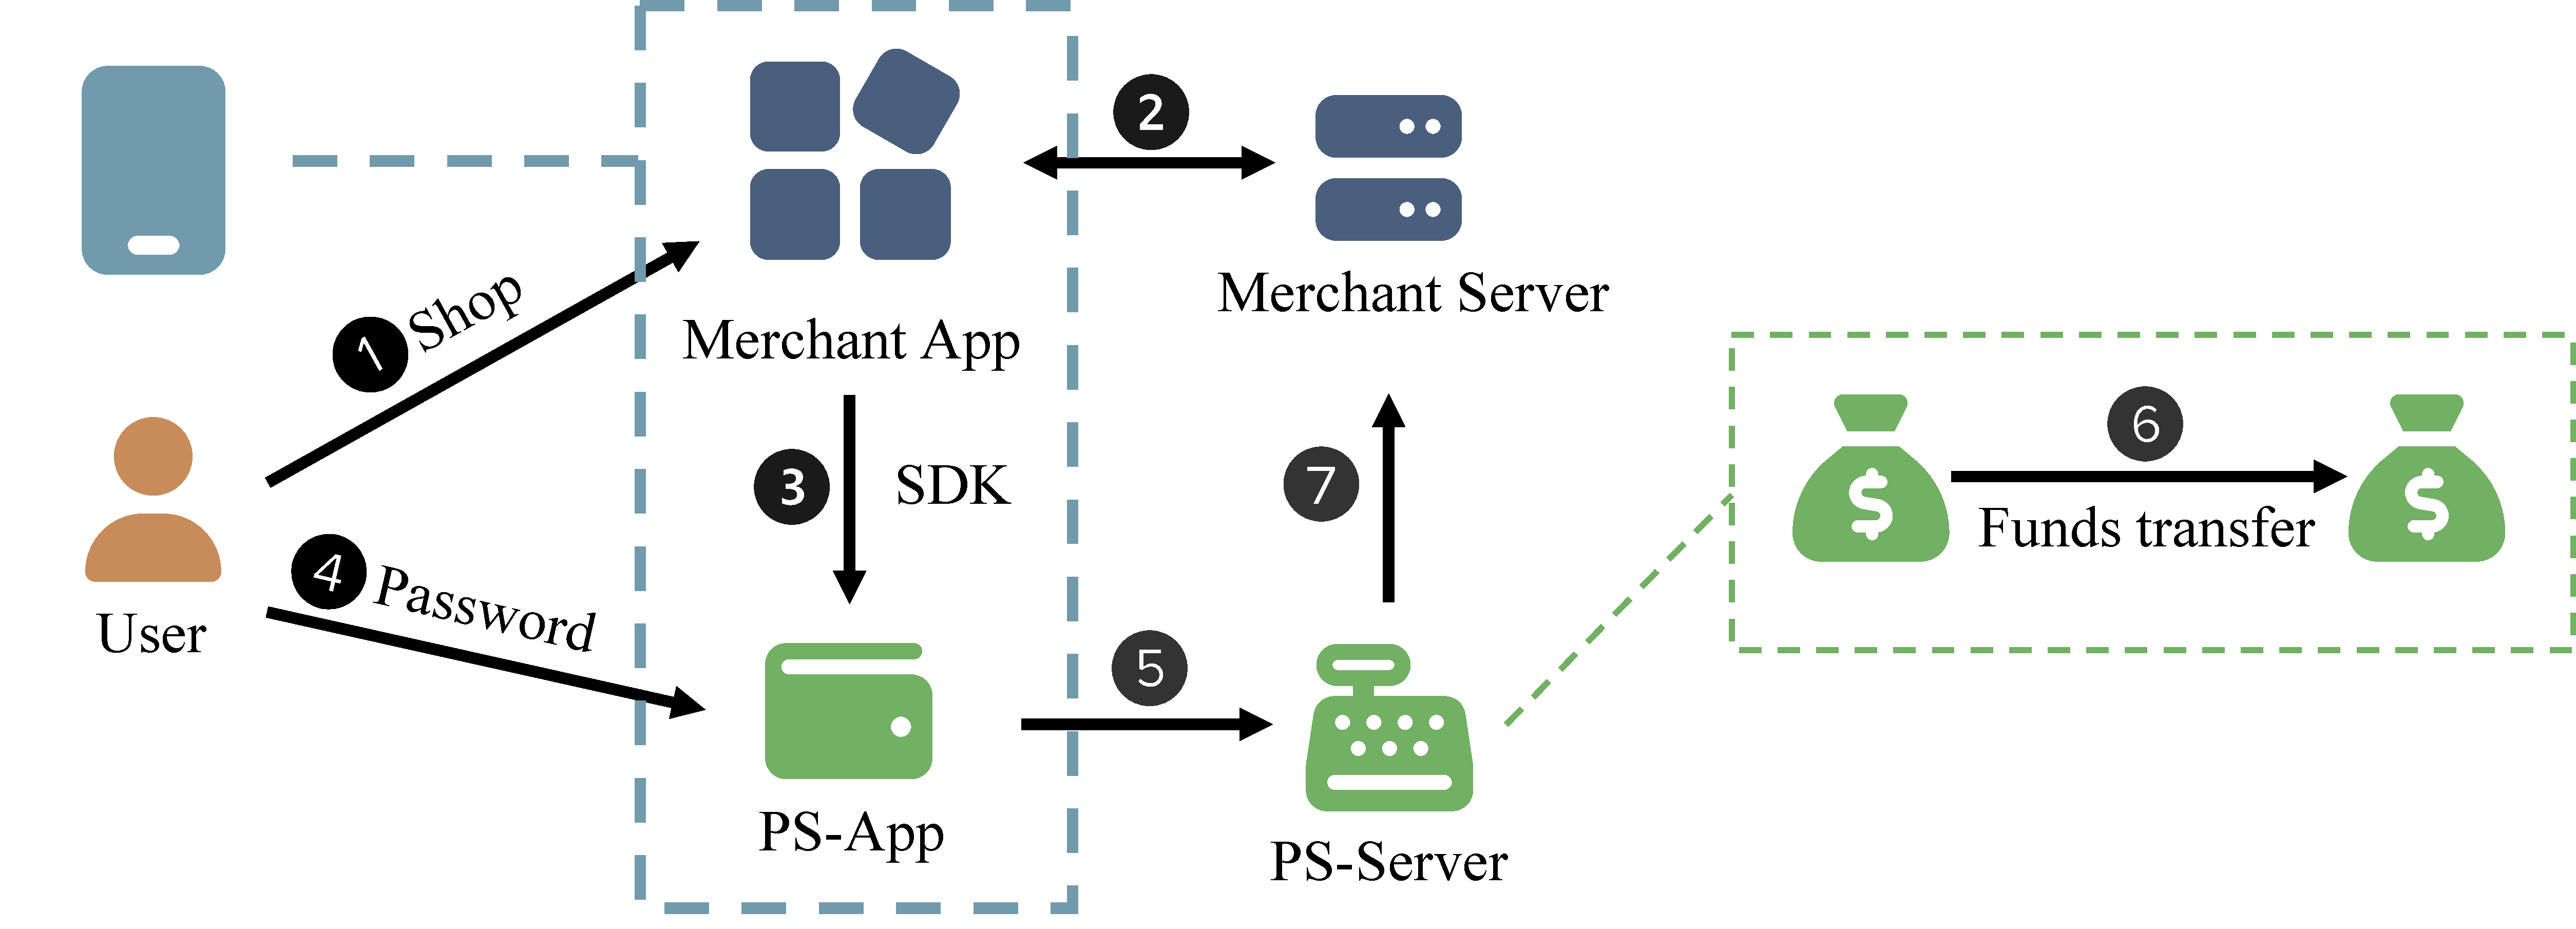
\includegraphics[width=\linewidth]{img/pays1.pdf}
    \caption{Payment Scenario \Rom{1} -- In-app Payment
    }
    \label{fig:inapp_payment}
\end{figure}

\begin{figure}[t]
    \centering
    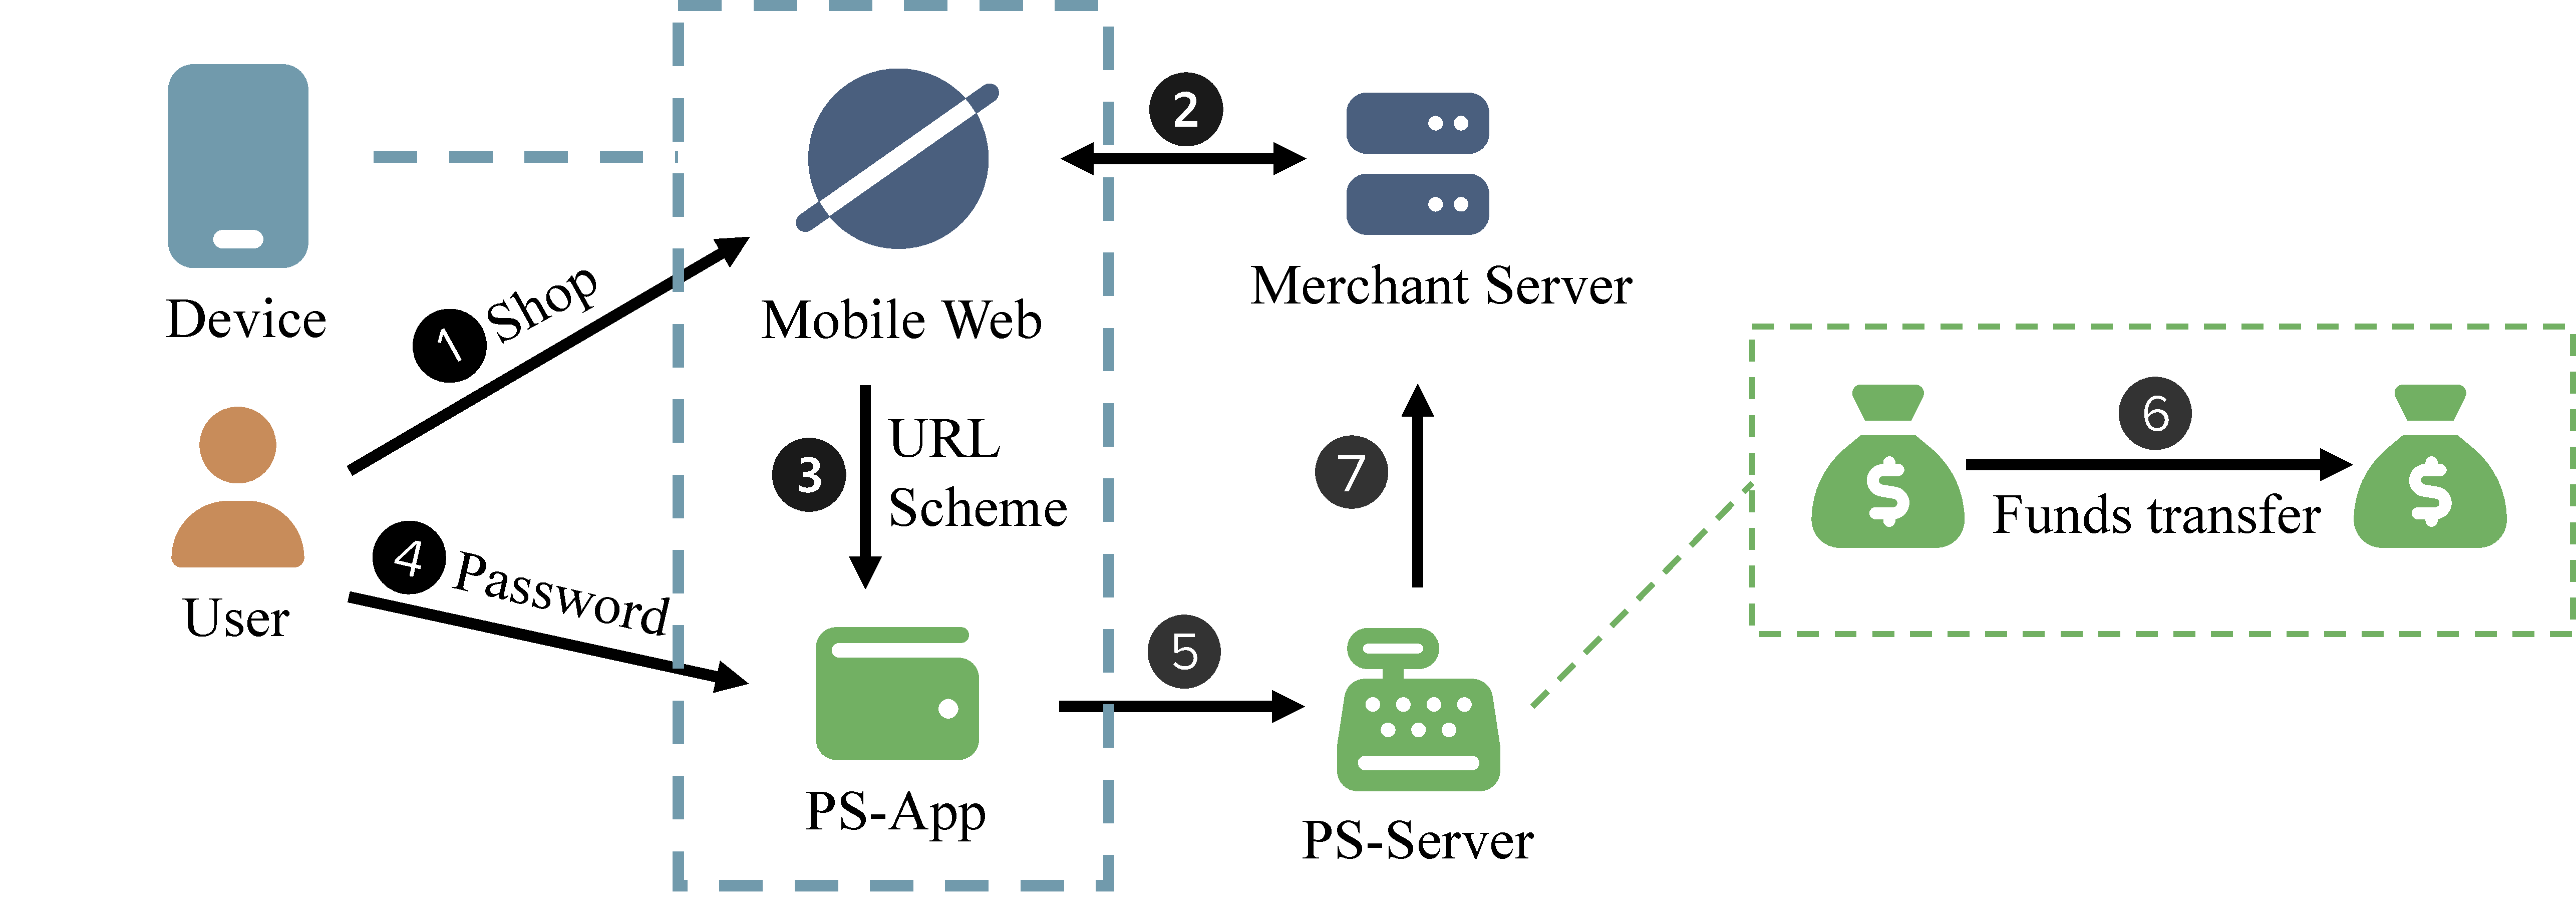
\includegraphics[width=\linewidth]{img/pays2.pdf}
    \caption{Payment Scenario \Rom{2} -- Mobile Web payment
    }
    \label{fig:mobile_web_payment}
\end{figure}

\begin{figure}[!h]
    \centering
    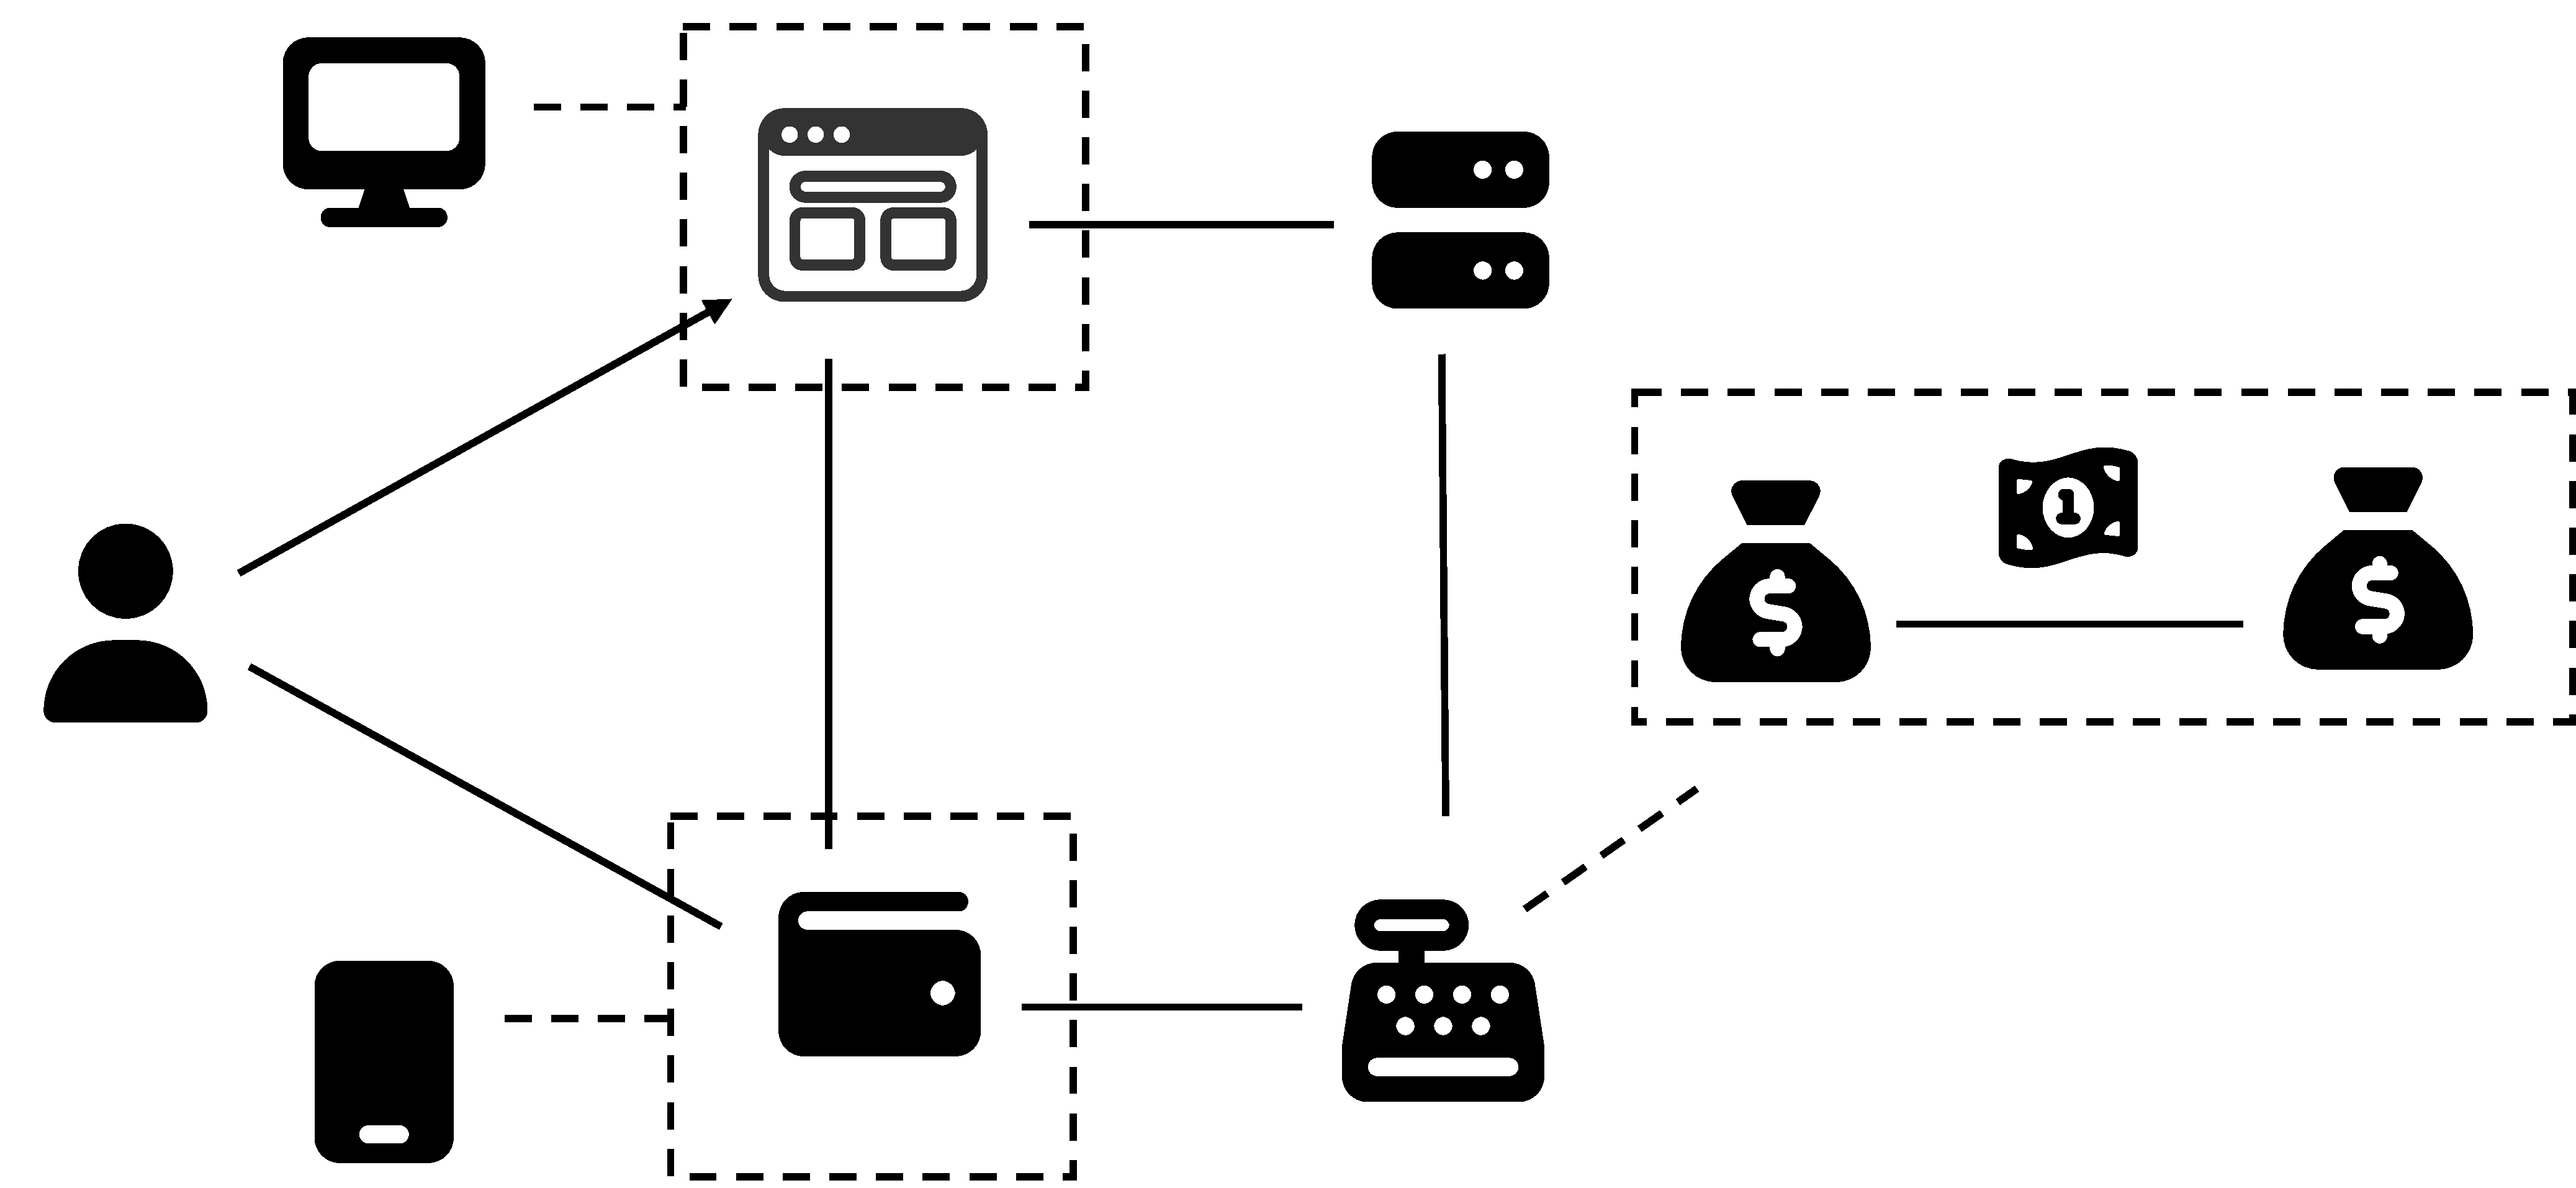
\includegraphics[width=\linewidth]{img/pays3.pdf}
    \caption{Payment Scenario \Rom{3} -- QR Code Payment
    }
    \label{fig:qr_code_payment}
\end{figure}



\newpage
\section{Alipay \& WeChat Pay Protocols}

We examined the actual protocol workflows of Alipay and WeChat Pay across three payment scenarios and documented them in detailed diagrams. 
Due to space constraints, we present a condensed version here.
The full versions are available in the open-source repository~\cite{third_payment_model_2026}.


\begin{figure*}[t]
    \centering

    \begin{subfigure}[b]{0.33\textwidth}
        \centering
        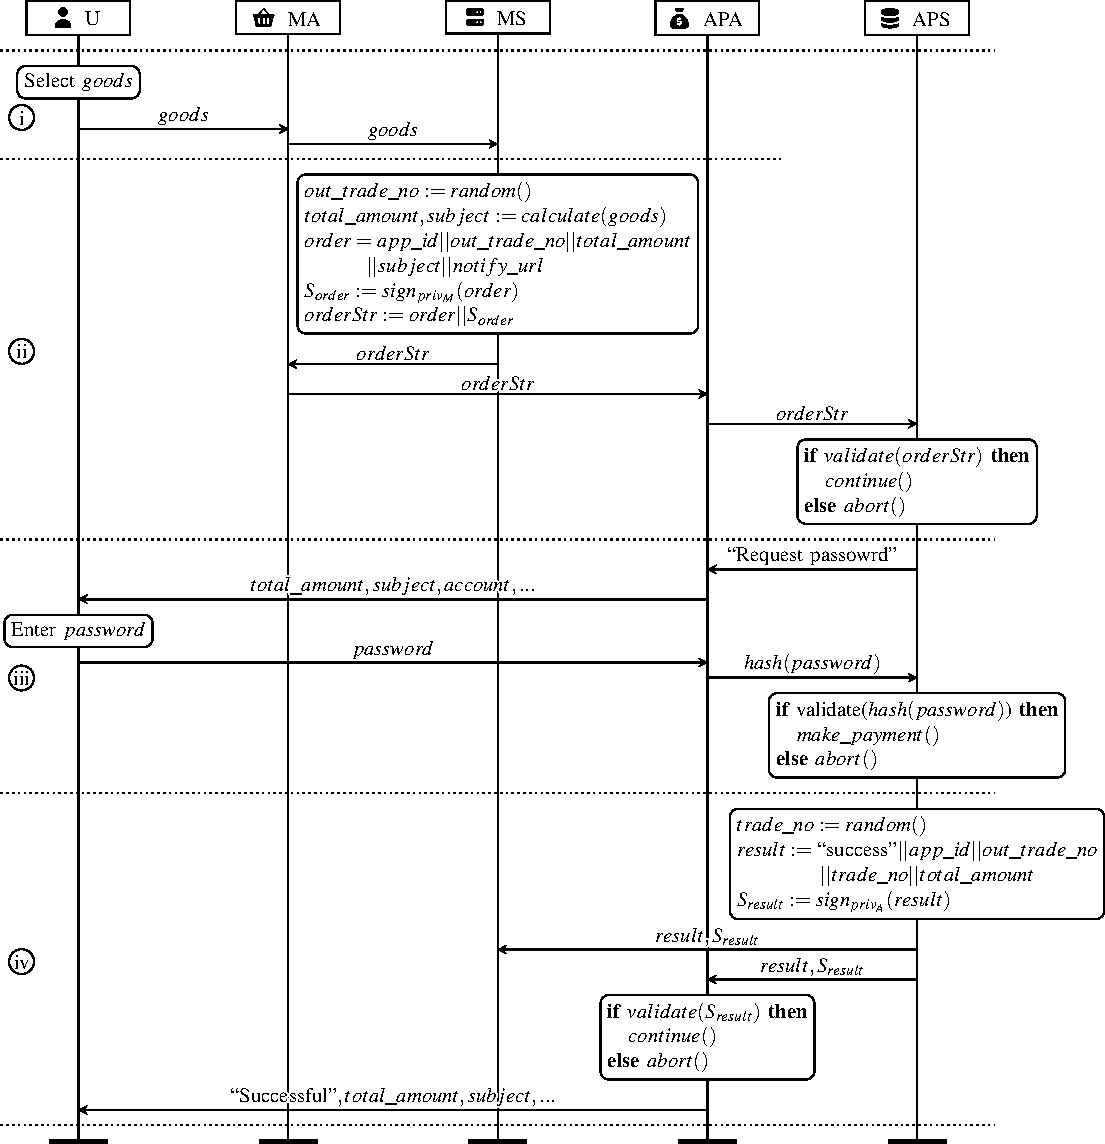
\includegraphics[width=\linewidth]{img/alipay_app.pdf}
        \caption{Alipay In-App Payment}
        \label{fig:alipay_in_app_payment}
    \end{subfigure}
    \hfill
    \begin{subfigure}[b]{0.33\textwidth}
        \centering
        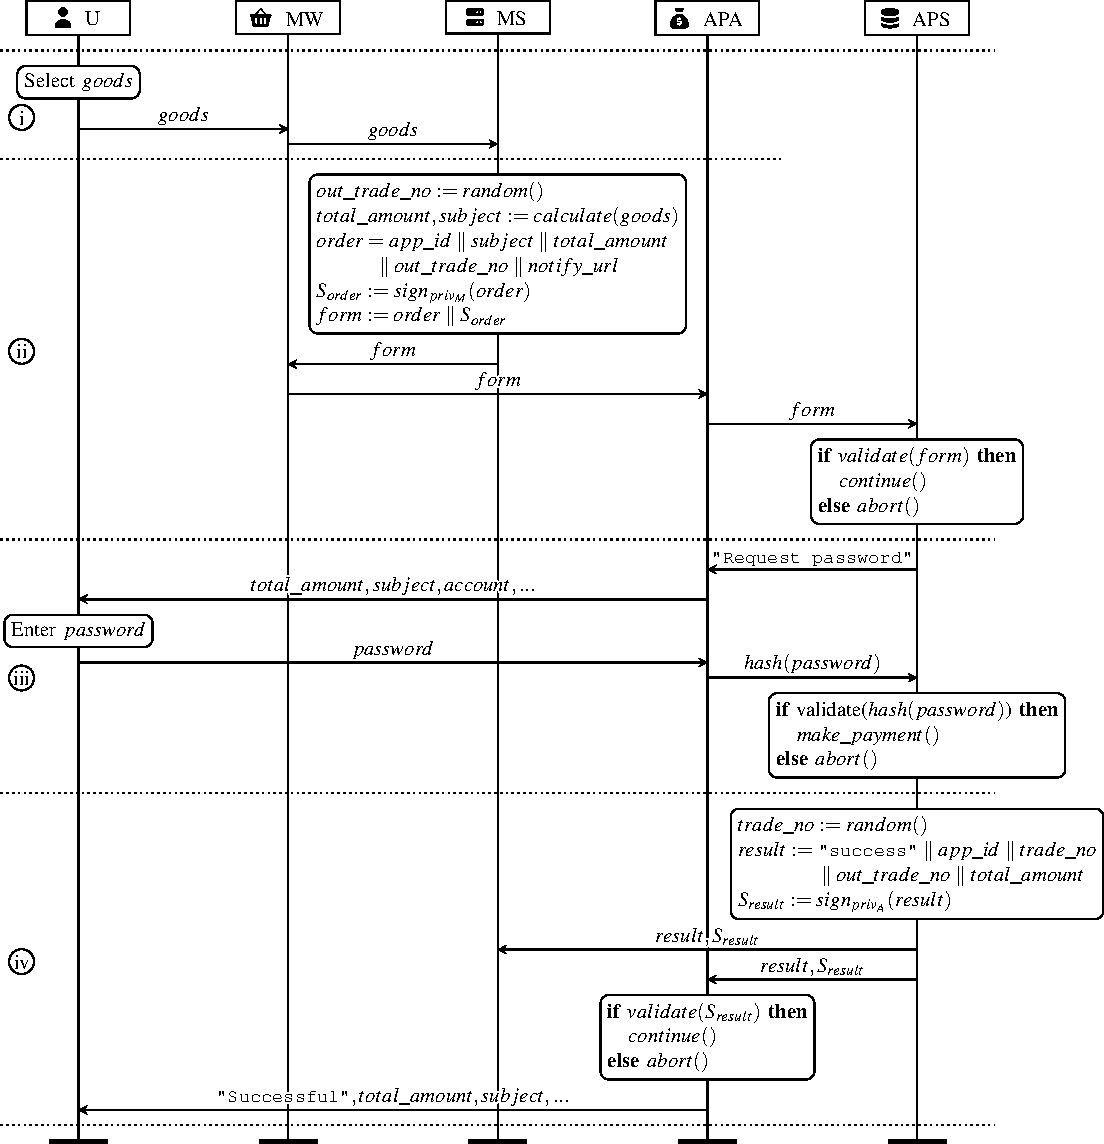
\includegraphics[width=\linewidth]{img/alipay_mobile_web.pdf}
        \caption{Alipay Mobile Web Payment}
        \label{fig:alipay_mobile_web_payment}
    \end{subfigure}
    \hfill
    \begin{subfigure}[b]{0.33\textwidth}
        \centering
        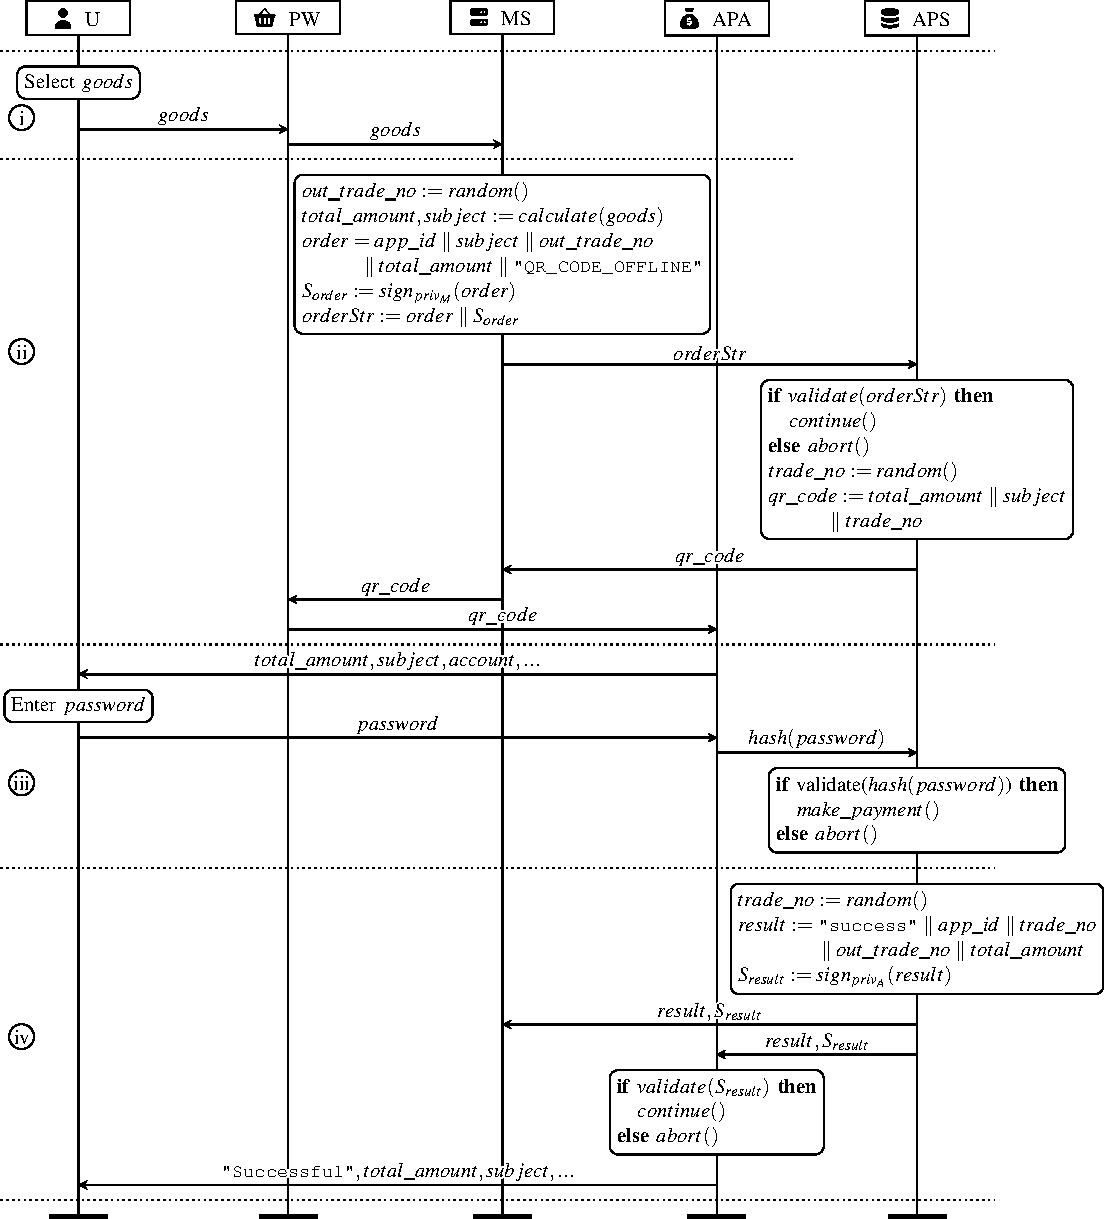
\includegraphics[width=\linewidth]{img/alipay_order_code.pdf}
        \caption{Alipay QR Code Payment}
        \label{fig:alipay_qr_code_payment}
    \end{subfigure}

    \caption{Alipay Payment Methods}
    \label{fig:alipay_payment_methods}
\end{figure*}

\begin{figure*}[t]
    \centering

    \begin{subfigure}[b]{0.33\textwidth}
        \centering
        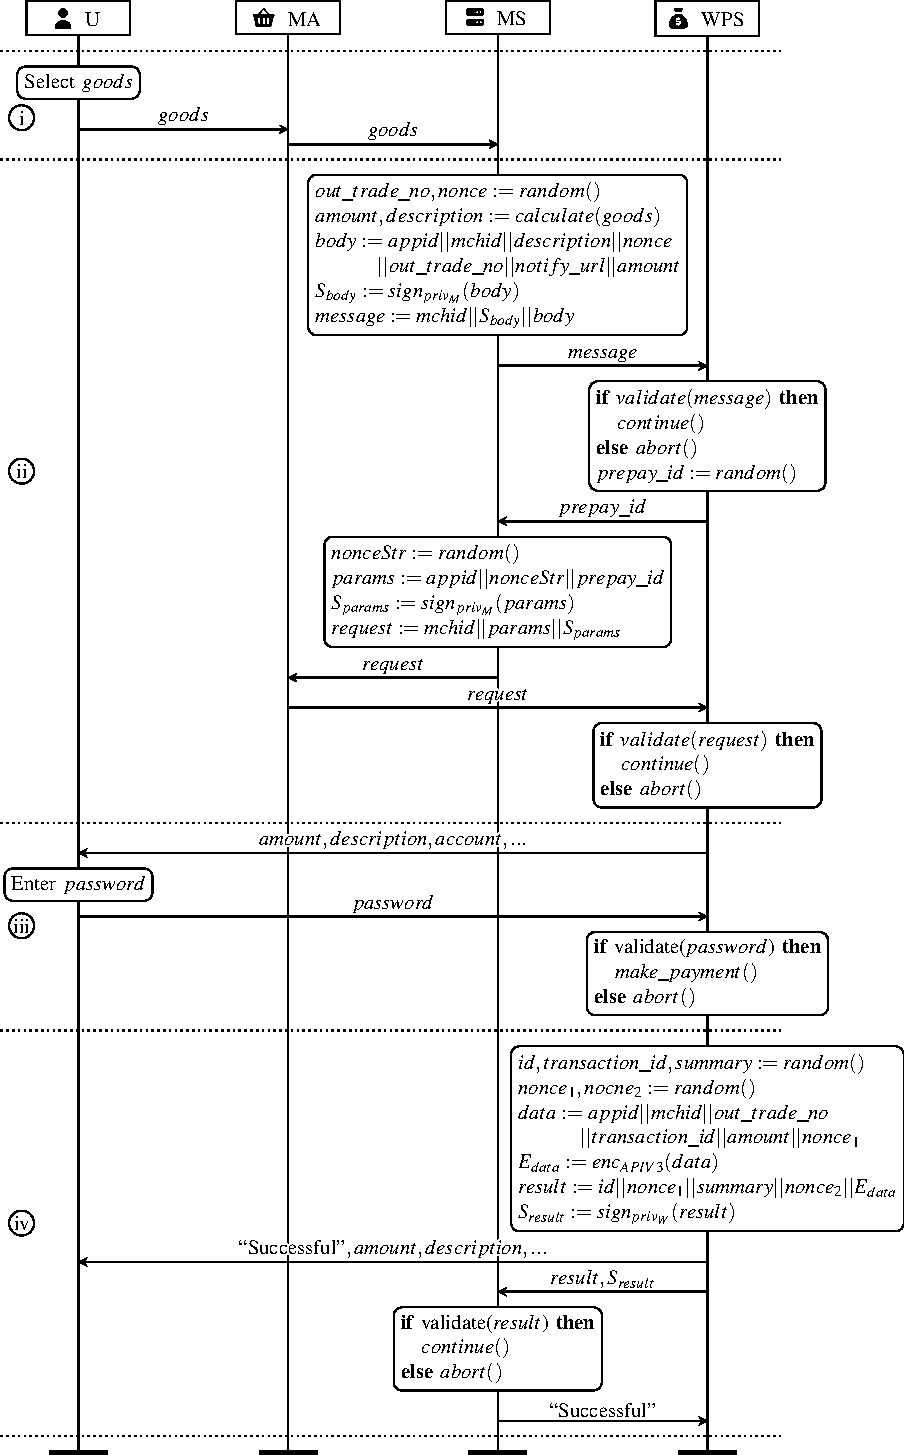
\includegraphics[width=\linewidth]{img/wechat_pay_app.pdf}
        \caption{In-App Payment}
        \label{fig:wechat_pay_in_app_payment}
    \end{subfigure}
    \hfill
    \begin{subfigure}[b]{0.33\textwidth}
        \centering
        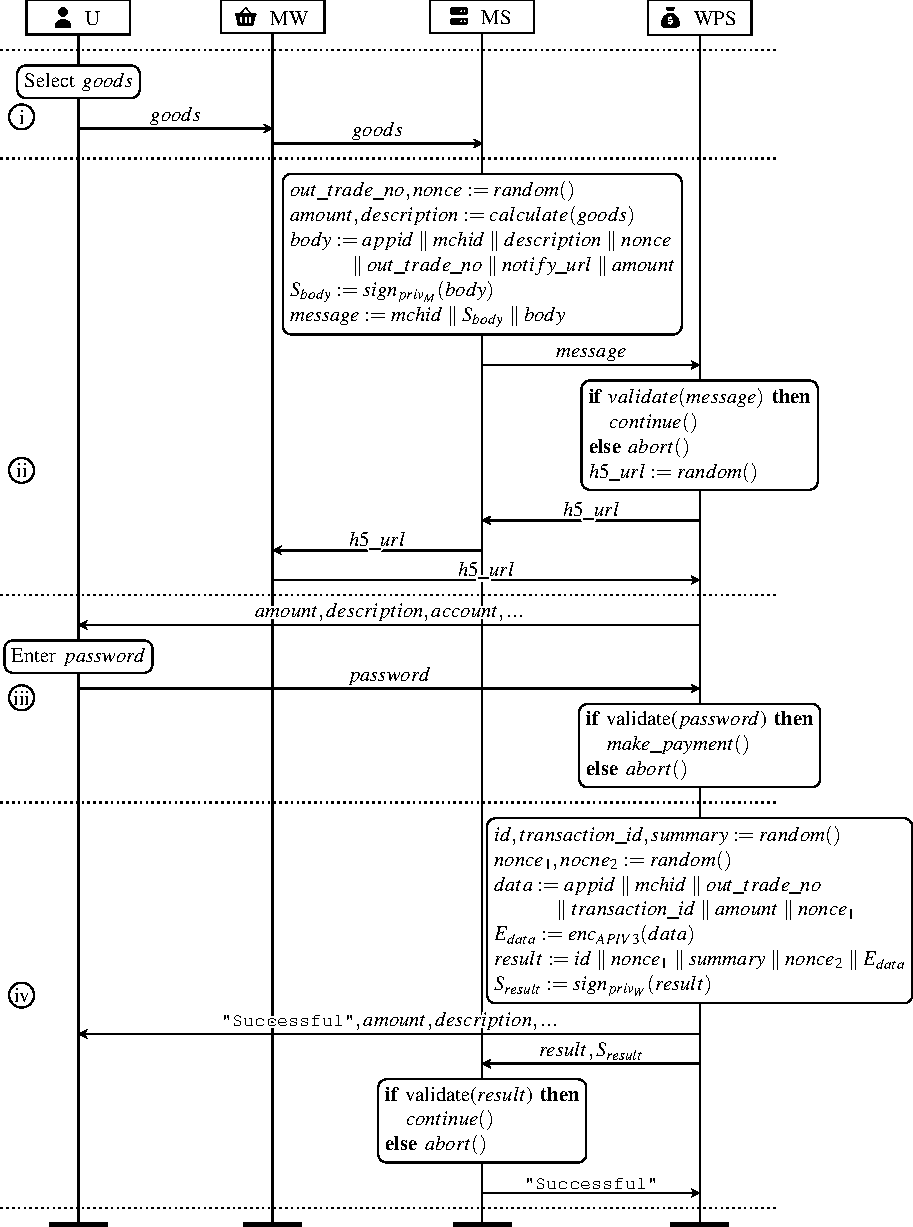
\includegraphics[width=\linewidth]{img/wechat_pay_h5.pdf}
        \caption{Mobile Web Payment}
        \label{fig:wechat_pay_mobile_web_payment}
    \end{subfigure}
    \hfill
    \begin{subfigure}[b]{0.33\textwidth}
        \centering
        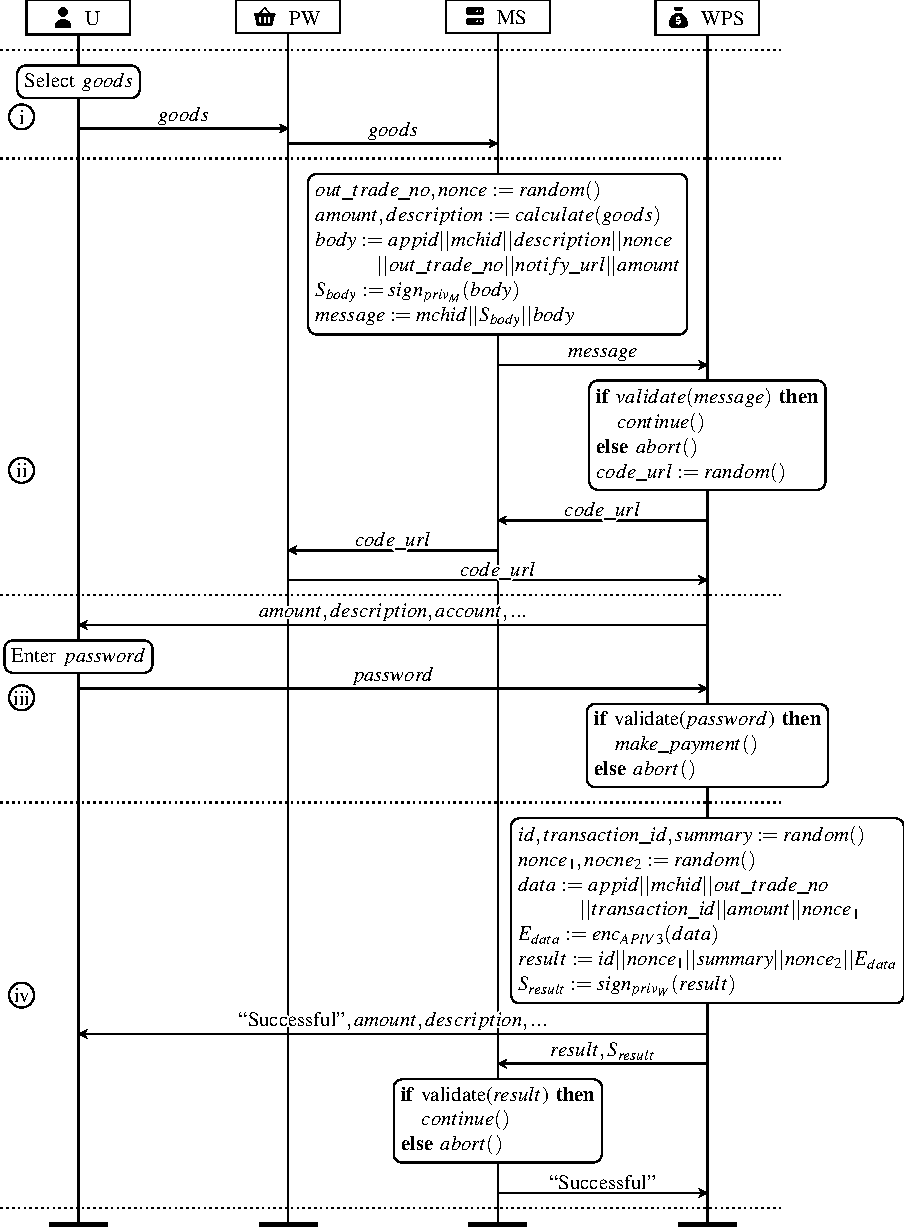
\includegraphics[width=\linewidth]{img/wechat_pay_native.pdf}
        \caption{QR Code Payment}
        \label{fig:wechat_pay_qr_code_payment}
    \end{subfigure}

    \caption{Wechat Pay Payment Methods}
    \label{fig:wechat_pay_payment_methods}
\end{figure*}

